\documentclass{acm_proc_article-sp}
\usepackage{graphicx}
\graphicspath{ {Image/} }
\DeclareGraphicsExtensions{.png}

\begin{document}

\title{Parallel Patterns using Heterogeneous Computing}
\subtitle{}
\numberofauthors{3} 
\author{
\alignauthor
Mr Andreas Vermeulen\\
\affaddr -\\
\affaddr {\small University of St Andrews}\\
\affaddr {\small Saint Andrews, Fife KY16 9AJ}\\
\affaddr -\\
\affaddr {\small University of Dundee}\\
\affaddr {\small Nethergate,Dundee DD1 4HN}\\
\affaddr -\\
\email{{\small a.f.vermeulen@dundee.ac.uk}}
\alignauthor
Dr Vladimir Janjic\\
\affaddr -\\
\affaddr {\small University of St Andrews}\\
\affaddr {\small Saint Andrews, Fife KY16 9AJ}\\
\affaddr -\\
\email{{\small vj32@st-andrews.ac.uk}}
\alignauthor
Mr Andy Cobley\\
\affaddr -\\
\affaddr {\small University of Dundee}\\
\affaddr {\small Nethergate, Dundee DD1 4HN}\\
\affaddr -\\
\email{{\small acobley@computing.dundee.ac.uk}}
}
\date{5 April 2015}
\maketitle
\begin{abstract}
\textit{Joint research project between University of St Andrews and University of Dundee for an enhancement of a Research Information Factory using heterogeneous computing and parallel knowledge-extraction patterns.}
\end{abstract}
\category{H.4}{Information Systems Applications}{Miscellaneous}
\terms{Theory, Framework, Application, Research, Hardware}
\keywords{\textit{knowledge-extraction, patterns, information factory, RIF, RIFF, RIFC ,heterogeneous computing, parallel patterns, cassandra, spark, opencl, fastflow, cuda, 3D torus network}}
\section{Introduction}
The demand for processing data into knowledge is exponentially increasing as new raw data sources appear and the volume of data they generate increases daily. The conversion of data into actionable knowledge is important for the future of modern society. Every aspect of our lives ranging from health care to shopping are now impacted by our ability to process more data per person per day. 
The increase of volume, variety, velocity and veracity is a major challenge to data scientists.
The volume can not process on a single storage system and now require to spread over multiple systems. 
The variety cause complexity in the processing to consolidate more data on same real world object. 
The speed or velocity of data creation is demanding more processing every second of the day. 
The veracity of the data requires that extra quality checks on data.
The trend over the last years is to build bigger and bigger data centers with massive energy requirements. This trend can not be sustain worldwide. Energy costs money and consumes natural resources that is getting more scares.

\textbf{\textit{Research goal is effective processing patterns with less energy cost.}}
\section{Background}
The research into heterogeneous computing using parallel patterns.
\subsection{Heterogeneous Computing}
Heterogeneous computing systems [11] uses more than one type of processors. Systems gain performance enhancements by the ability to utilise dissimilar processors to execute common processing requirements. Using central processing unit (\textit{CPU}), graphical processing unit (\textit{GPU}) and field-programmable gate array (\textit{FPGA}) processor that enable effective processing at low energy requirements.
The central processing unit (\textit{CPU}) is designed with few cores optimised for sequential serial processing patterns that requires large amounts of control changes. The graphical processing unit (\textit{GPU}) is designed as a massively parallel architecture of thousands of smaller, efficient cores handling multiple tasks simultaneously. The spesilised Application-Specific Integrated Circuit (\textit{ASIC}) solution is capable of performing fixed spesific tasks like network connectivity, mapping information. Field-Programmable Gate Array (\textit{FPGA}) is a set of programmable logic blocks and programmable interconnects allow the same FPGA to be used in many different applications. Heterogeneous uses them together as one unit.
\subsection{Parallel Patterns}
Patterns is the fundimental programming building blocks of data processing requirement. Heterogeneous computing changes the design and implimentation of common parallel patterns (task parallelism, pipelines, recursive splitting and geometric decomposition of data processing). We require new knowledge-extraction patterns using common strategies (actors, shared queue, fork/join, loop parallelism and master/worker) with libraries (CUDA [7], OpenCL[5][8][9][13], FastFlow [6] and ZeroMQ [10]).
\subsection{Efficiency and Energy-awareness}
The increasing drive for processing power demand increase energy levels to perform tasks. Our research targets efficiency in terms of processing time, programming effort, energy-awareness for each design pattern. Research calculates efficiency of processing in Floating-point Operations Per Second per Watt (\textit{FLOP/S/W}). 
\subsection{Research Information Factory}
The Research Information Factory (\textit{RIF}) is a processing appliance consisting of a framework and a cluster that supports the conversion of raw research data into knowledge using parallel patterns. 
\subsubsection{RIF Framework}
The Research Information Factory Framework (\textit{RIFF}) is a data processing framework that was designed 
during the period 2006 to 2011 and officially published as part of a MSc in Business Intelligence project (2012) and adapted during a Pg Cert in Data Science (2013) [15] to support unstructured and structured data patterns.  
The framework contains a set of guidelines to process data into knowledge. 
Framework uses a five layer process Research Layer (spesific research requirements), Utility Layer (common processing utilities), Audit, Balance and Control Layer (schedule jobs, collect audits, control patterns)
Operational Management Layer (active processing controls) Functional Layer supports the core processing pattern of \textbf{R}etrieve-\textbf{A}ssess-\textbf{P}rocess-\textbf{T}ransform-\textbf{O}rganise-\textbf{R}eport (\textit{R-A-P-T-O-R}). 
\begin{figure}
  \centering
  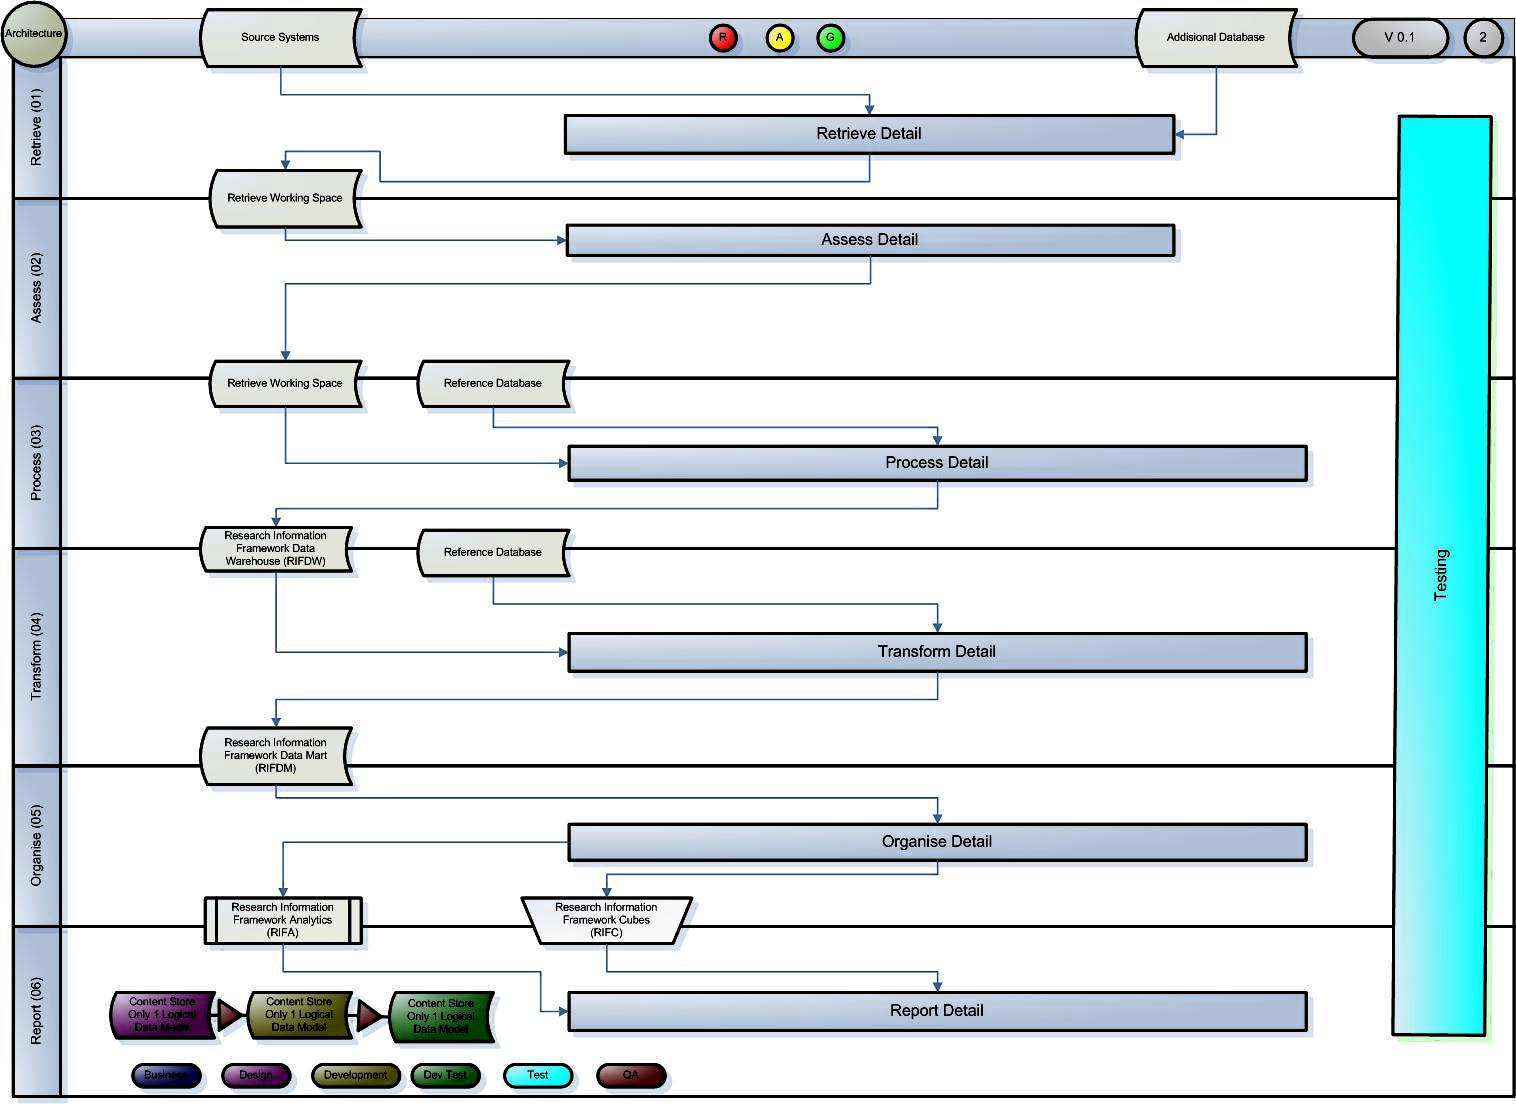
\includegraphics[width=5cm]{RIFF}
  \caption{Research Information Factory Framework}
\end{figure}
\subsubsection{RIF Cluster}
The Research Information Factory Cluster (\textit{RIFC}) is a 3D torus connected cluster appliance using commondity computer equipment to process the RIFF parallel patterns. This new custom parallel cluster appliance design [15] (Synaptic Assimilator) supports the RIFF. The cluster supports a Cassandra database [2] and a Spark Processing Engine [12] to handle the scalability and high availability data processing to match the parallel patterns requirements for data sources of a size larger than what a single system can handle.
\section{Proposed Solution}
The reearch will develop new parallel patterns for knowledge extraction, new mechanisms for storing and extracting data while using minimum amounts of energy.
The research over next year covers three stages:
\subsection{Heterogeneous systems.}
The research will study the fundamental behavior of a selection of heterogeneous computing components as implimented in a nVidia Jetson TK1 development kit. [4]
\subsection{Parallel patterns for data processing}
The behavior is evaluated on a basis of a fixed size data set processed via a spesific parallel pattern changing parameters like combinations of CPU, GPU with different clock speeds, memory allocations and measuring time to complete task, energy requirements and effort in amount of code required for each parallel pattern and heterogeneous computing combination. 
\subsection{Research Information Factory Cluster}
The Research Information Factory Cluster (\textit{RIFC}) is a 3D torus connected cluster appliance using commondity computer equipment, a Cassandra database [2] and a Spark Engine [12] to handle the scalability and high availability data processing from systems like nVidia Jetson TK1 [4] and Tilera TILE-Mx100 processor [14].
\section{Conclusion}
The research goal is to do more processing with less energy. Heterogeneous systems with parallel patterns is currently the optimum option to acheve the goal. 
\section{References}
\begin{small}
[1] Ashfaq A. Khokhar, Viktor K. Prasanna,Muhammad E. Shaaban, Cho-Li Wang, (1993); Heterogeneous Computing: Challenges and Opportunities. 

[2] Cassandra, (2014), Apache Cassandra; http://cassandra.apache.org/ 

[3] Datastax, (2014), Getting Started with Apache Spark and Cassandra; 
http://planetcassandra.org/getting-started-with-apache-spark-and-cassandra/
 
[4] NVIDIA Jetson TK1, (2014), NVIDIA Jetson TK1 development kit.

[5] Khronos, (2014), OpenCL; https://www.khronos.org/opencl/

[6] M. Aldinucci, M. Danelutto, P. Kilpatrick, and M. Torquati, (2011), 
FastFlow: high-level and efficient streaming on multi-core in Programming Multi-core and Many-core Computing System.

[7] nVidia, (2014), CUDA Tool Kit.

[8] OpenCL 1.2, (2011), OpenCL 1.2 Reference Card.

[9] OpenCL 2.0, (2013), OpenCL 2.0 Reference Card.

[10] Pieter Hintjens (2014), ØMQ - The Guide.

[11] Qiang Wu,Yajun Ha ; Kumar, A. ; Shaobo Luo ; Ang Li ; Mohamed, S., (2014), A heterogeneous platform with GPU and FPGA for power efficient high performance computing.

[12] Spark, (2014), Spark Lightning-fast cluster computing.

[13] Stone, J.E. ; Gohara, D. ; Guochun Shi,(2010), OpenCL: A Parallel Programming Standard for Heterogeneous Computing Systems, Comput. Sci. Eng. 12, 66 (2010).

[14] Tilera, (2007), Tilera Processor Family.

[15] Yuichiro Ajima, Shinji Sumimoto, Toshiyuki Shimizu, (2009), "Tofu: A 6D Mesh/Torus Interconnect for Exascale Computers," IEEE Computer, vol. 42, no. 11, November 2009, pp. 36-40.
\end{small}
\end{document}
